The purpose of this section is to answer both the checkpoint and report
questions of the lab, as well as discuss any relevant results obtained during the experiences.

\subsection{SYSTEM 1: Analog Reading and LED Bar}

\begin{enumerate}

    \item \textbf{Checkpoint 1: Run the simulation.}
    \par \vspace{0.15cm}
    Shown in Figure~\ref{fig:1}

    \begin{figure}[htbp]
        \centering
        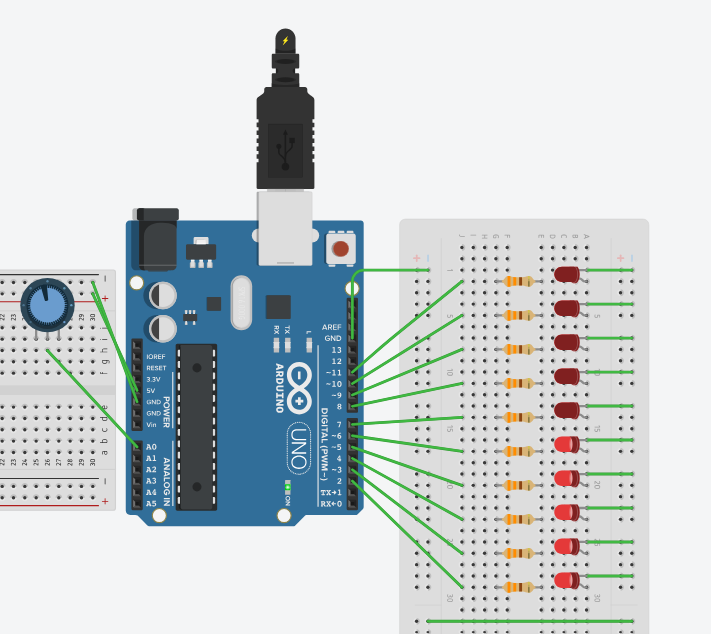
\includegraphics[width=1\linewidth]{img/checkpoint1.png}
        \caption{Tinkercad Simulation of System 1.}\label{fig:1}
    \end{figure}

    \begin{itemize}
        \item The corresponding Tinkercad implementation is available at: 
        \href{https://www.tinkercad.com/things/9Q1Zr4doDzV-barrita/editel?returnTo=https%3A%2F%2Fwww.tinkercad.com%2Fthings%2F9Q1Zr4doDzV-barrita&sharecode=omk7smMwn-rR2kLFnrSrMlOvJsiKk6Njiqra4cd1KIA}{view Tinkercad simulation}.
    \end{itemize}

    \item \textbf{Checkpoint 2: Carry out the physical implementation and record a demonstration video.}

    \begin{itemize}
        \item The physical implementation is demonstrated in the following video:
        \href{https://drive.google.com/file/d/1lb-KOxjORNLkK3BwuQjImiEukMwBvksX/view?usp=drive_link}{view video demonstration}.
    \end{itemize}

    \item \textbf{Flowchart.}
    \par \vspace{0.15cm}
    Shown in Figure~\ref{fig:2}

    \begin{figure}[htbp]
        \centering
        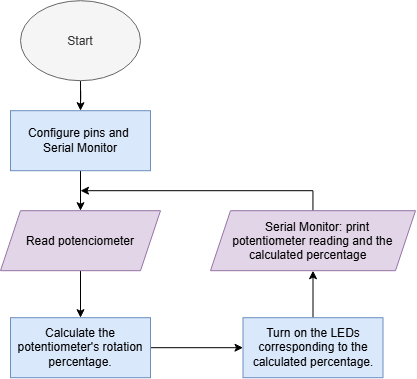
\includegraphics[width=1\linewidth]{img/diagrama_flujo-sistema1.drawio.png}
        \caption{Flowchart of System 1.}\label{fig:2}
    \end{figure}


    \item \textbf{Block Diagram.}
    \par \vspace{0.15cm}
    Shown in Figure~\ref{fig:3}

    \begin{figure}[htbp]
        \centering
        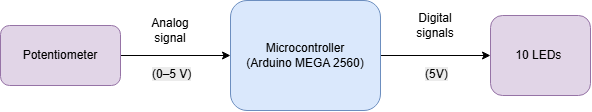
\includegraphics[width=1\linewidth]{img/diagrama_bloques-sistema1.drawio.png}
        \caption{Block Diagram of System 1.}\label{fig:3}
    \end{figure}

\end{enumerate}


\subsection{SYSTEM 2: Ambient Light Sensor and System Monitoring}

\begin{enumerate}

    \item \textbf{Checkpoint 3: Run the simulation.}
    \par \vspace{0.15cm}
    Shown in Figure~\ref{fig:4}
    \begin{figure}[htbp]
        \centering
        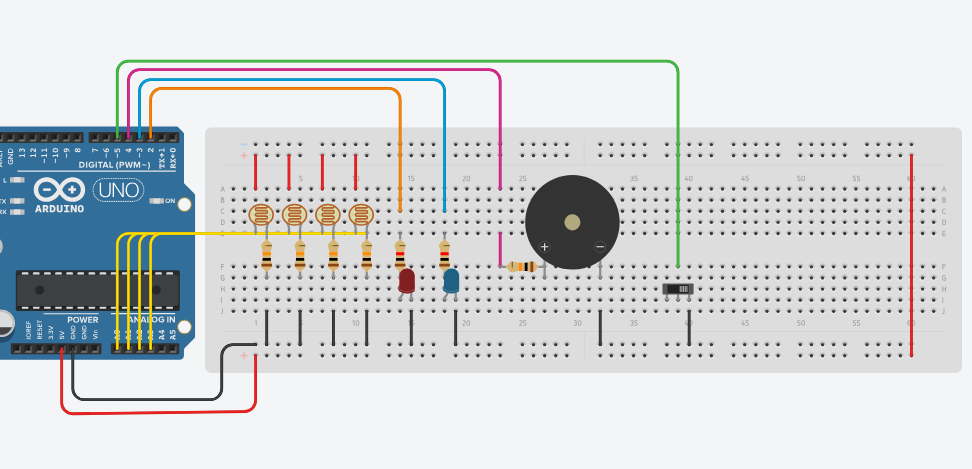
\includegraphics[width=1\linewidth]{img/checkpoint3.png}
        \caption{Tinkercad Simulation of System 2.}\label{fig:4}
    \end{figure}

    \begin{itemize}
        \item The corresponding Tinkercad implementation is available at: 
        \href{https://www.tinkercad.com/things/aPN2onW6buG-sensor-de-luz/editel?returnTo=https%3A%2F%2Fwww.tinkercad.com%2Fdashboard&sharecode=Dx6uvHBQzcoP6c_kkDWgllSTkm9deS76eTwB516JIxo}{view Tinkercad simulation}.
    \end{itemize}

    \item \textbf{Checkpoint 4: Carry out the physical implementation and record a demonstration video.}

    \begin{itemize}
        \item The physical implementation is demonstrated in the following video: 
        \href{https://drive.google.com/file/d/1jt73U9jTPeC79SI0v_eQKez06liPBJ8F/view?usp=drive_link}{view video demonstration}.
    \end{itemize}

    \item \textbf{Flowchart.}
    \par \vspace{0.15cm}
    Shown in Figure~\ref{fig:5}
    \begin{figure}[htbp]
        \centering
        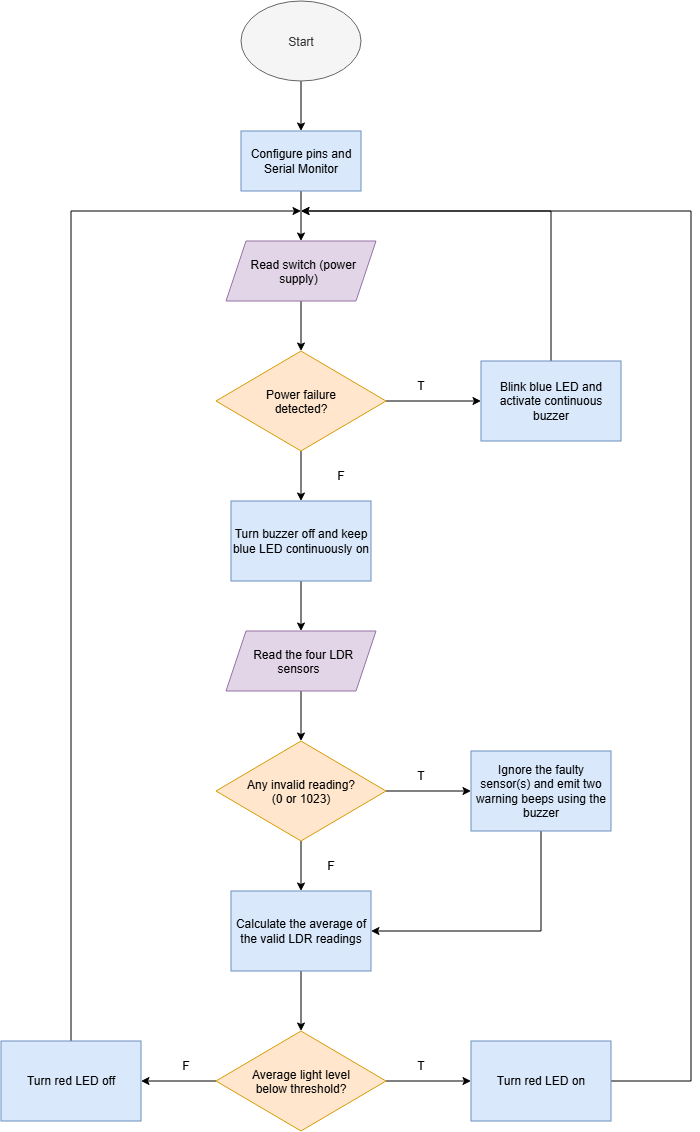
\includegraphics[width=1\linewidth]{img/diagrama_flujo-sistema2.drawio.png}
        \caption{Flowchart of System 2.}\label{fig:5}
    \end{figure}


    \item \textbf{Block Diagram.}
    \par \vspace{0.15cm}
    Shown in Figure~\ref{fig:6}
    \begin{figure}[htbp]
        \centering
        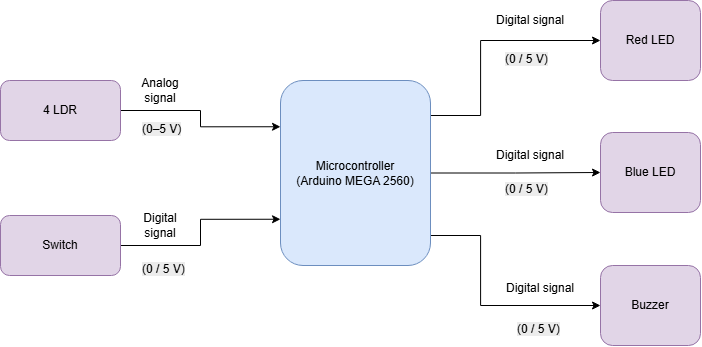
\includegraphics[width=1\linewidth]{img/diagrama_bloques-sistema2.drawio.png}
        \caption{Block Diagram of System 2.}\label{fig:6}
    \end{figure}

\end{enumerate}



\subsection{SYSTEM 3: Occupancy Control and Environmental Safety}

\begin{enumerate}

    \item \textbf{Checkpoint 5: Run the simulation.}
    \par \vspace{0.15cm}
    Shown in Figure~\ref{fig:7}
    \begin{figure}[htbp]
        \centering
        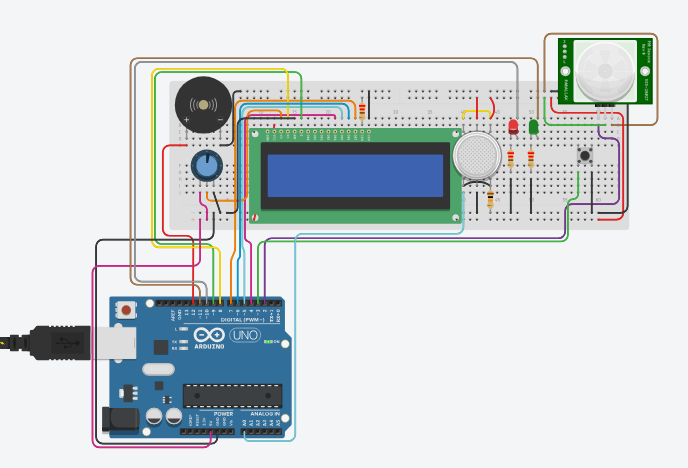
\includegraphics[width=1\linewidth]{img/checkpoint5.png}
        \caption{Tinkercad Simulation of System 3.}\label{fig:7}
    \end{figure}

    \begin{itemize}
        \item The corresponding Tinkercad implementation is available at: 
        \href{https://www.tinkercad.com/things/1NYTk80ATw5-exquisite-kieran-crift/editel?returnTo=https%3A%2F%2Fwww.tinkercad.com%2Fdashboard&sharecode=QWmfLSWPRl3msW4cpbzg-Cnt4fUuPdA9AaguGxM3MnM}{view Tinkercad simulation}.
    \end{itemize}

    \item \textbf{Checkpoint 6: Carry out the physical implementation and record a demonstration video.}

    \begin{itemize}
        \item The physical implementation is demonstrated in the following video: 
        \href{https://drive.google.com/file/d/14y4siQy6AZoSGVfKCnuHXg24x8amtlW1/view?usp=drive_link}{view video demonstration}.
    \end{itemize}

    \item \textbf{Flowchart.}
    \par \vspace{0.15cm}
    Shown in Figure~\ref{fig:8}
    \begin{figure}[htbp]
        \centering
        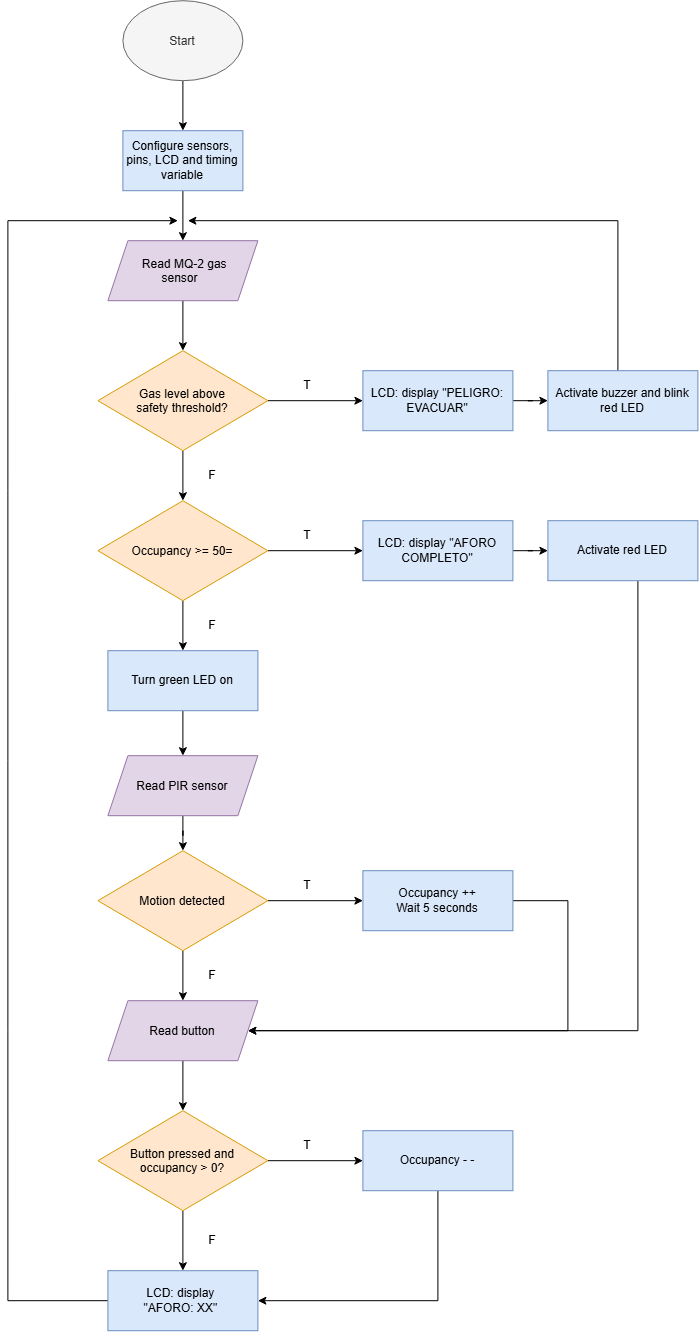
\includegraphics[width=1\linewidth]{img/diagrama_flujo-sistema3.drawio.png}
        \caption{Flowchart of System 3.}\label{fig:8}
    \end{figure}


    \item \textbf{Block Diagram.}
    \par \vspace{0.15cm}
    Shown in Figure~\ref{fig:9}
    \begin{figure}[htbp]
        \centering
        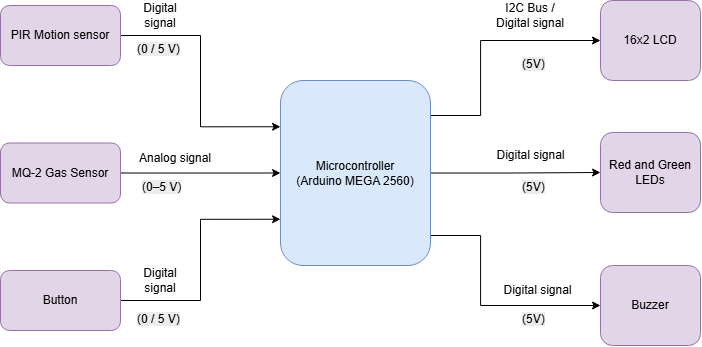
\includegraphics[width=1\linewidth]{img/diagrama_bloques-sistema3.drawio.png}
        \caption{Block Diagram of System 3.}\label{fig:9}
    \end{figure}

\end{enumerate}




\subsection{SYSTEM 4: Multiparameter Monitoring Station}

\begin{enumerate}

    \item \textbf{Checkpoint 7: Carry out the physical implementation and record a demonstration video.}

    \begin{itemize}
        \item The physical implementation is demonstrated in the following video: 
        \href{https://drive.google.com/file/d/1NKe_jgmIHQmVLyjyyOHRuUke2AN0VuaS/view?usp=drive_link }{view video demonstration}.
    \end{itemize}

    \item \textbf{Flowchart.}
    \par \vspace{0.15cm}
    Shown in Figure~\ref{fig:10}
    \begin{figure}[htbp]
        \centering
        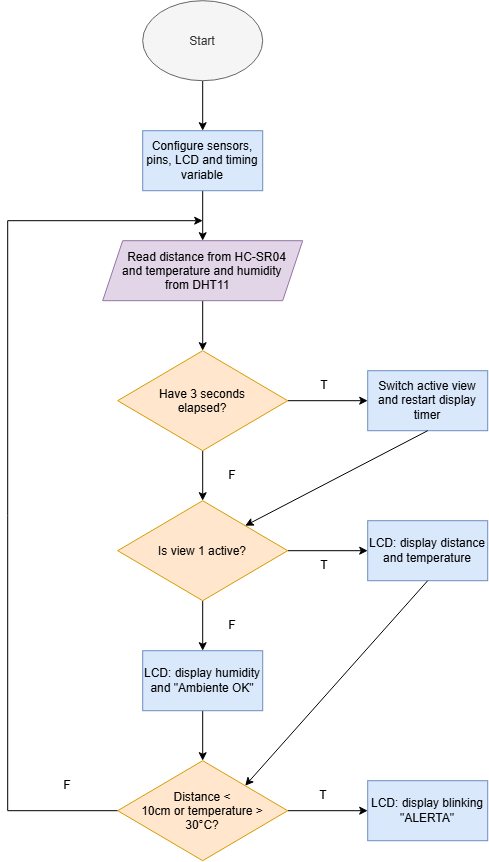
\includegraphics[width=1\linewidth]{img/diagrama_flujo-sistema4.drawio.png}
        \caption{Flowchart of System 4.}\label{fig:10}
    \end{figure}


    \item \textbf{Block Diagram.}
    \par \vspace{0.15cm}
    Shown in Figure~\ref{fig:11}
    \begin{figure}[htbp]
        \centering
        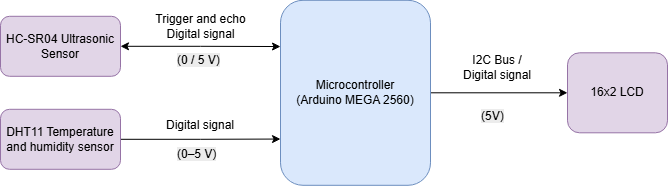
\includegraphics[width=1\linewidth]{img/diagrama_bloques-sistema4.drawio.png}
        \caption{Block Diagram of System 4.}\label{fig:11}
    \end{figure}

\end{enumerate}



\subsection{SYSTEM 5. Starting a DC Motor with Arduino}

\begin{enumerate}
    \item \textbf{What happens in your simulation with the Arduino? Is there any irregular behavior?}
    \par \vspace{0.15cm}
    No irregular behavior was observed during the initial simulation. The motor turned on when the voltage 
    selected using the potentiometer was between $3$ and $5\,\mathrm{V}$, as required. Shown in Figure~\ref{fig:12}
    
    \begin{figure}[htbp]
        \centering
        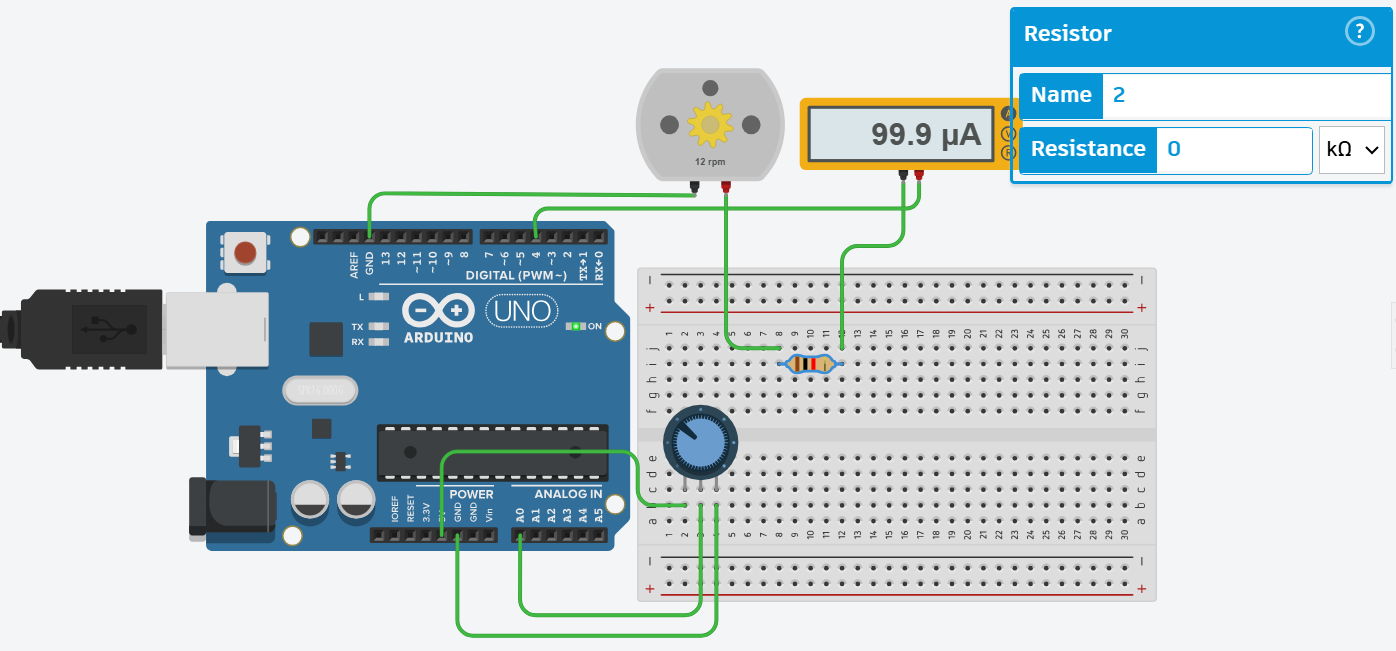
\includegraphics[width=1\linewidth]{img/checkpoint5-1.png}
        \caption{Initial System 5 simulation in Tinkercad.}\label{fig:12}
    \end{figure}
    
    \item \textbf{What is the current drawn by the motor during operation? (Use a measuring tool).}
    \par \vspace{0.15cm}
    The current measured during motor operation in the simulation was $99.9\,\mu\mathrm{A}$. Shown in Figure~\ref{fig:12}
    
    \item \textbf{What is the motor speed?}
    \par \vspace{0.15cm}
    The motor speed displayed in the initial simulation was $12\,\mathrm{rpm}$. Shown in Figure~\ref{fig:12}

    \item \textbf{Connect a $1\,\mathrm{k}\Omega$ resistor in series between the digital pin and the positive terminal of 
    the DC motor. Does the motor operate normally or show any irregular behavior? What is its speed?}
    \par \vspace{0.15cm}
    After adding the $1\,\mathrm{k}\Omega$ resistor, the motor continued to rotate at $12\,\mathrm{rpm}$ when the 
    potentiometer voltage was between $3$ and $5\,\mathrm{V}$. No visible irregular behavior was observed in the simulation.
    The current shown in the screenshot decreased slightly to $97.9\,\mu\mathrm{A}$. Shown in Figure~\ref{fig:13}

    \begin{figure}[htbp]
        \centering
        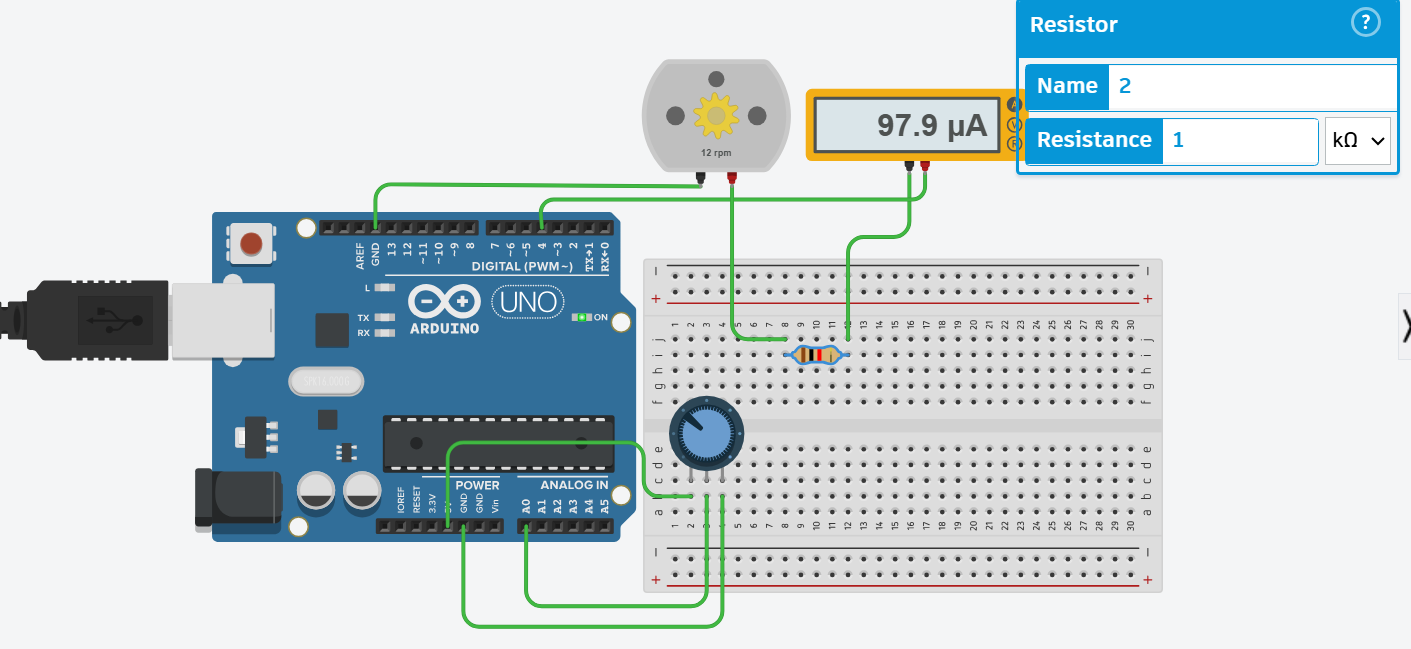
\includegraphics[width=1\linewidth]{img/checkpoint5-2.png}
        \caption{DC motor simulation with a $1\,\mathrm{k}\Omega$ series resistor.}\label{fig:13}
    \end{figure}

    \item \textbf{Connect the Arduino's $5\,\mathrm{V}$ pin directly to the positive terminal of the motor. 
    Does the motor operate normally or show any irregular behavior? What is its speed?}
    \par \vspace{0.15cm}
    Connecting the motor directly to the $5\,\mathrm{V}$ pin produced a substantial increase in speed compared 
    with the previous configurations. The recorded value was $9994\,\mathrm{rpm}$, compared with the initial 
    $12\,\mathrm{rpm}$. This change shows that the motor behaved differently when supplied directly from the $5\,\mathrm{V}$ pin.
    Shown in Figure~\ref{fig:14}

    \begin{figure}[htbp]
        \centering
        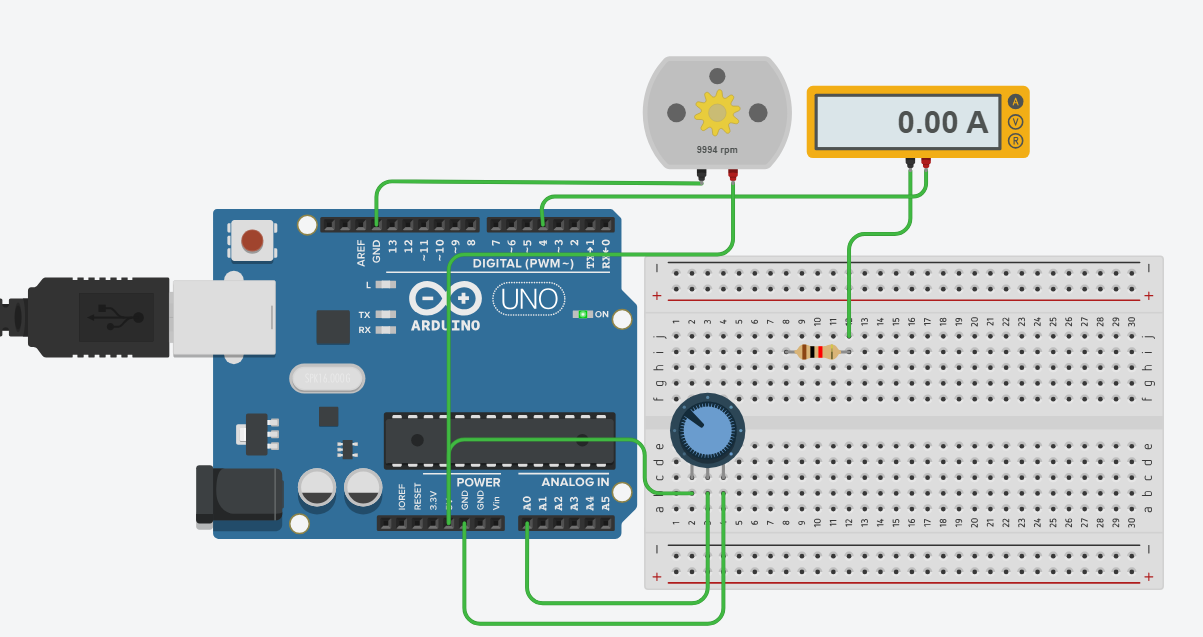
\includegraphics[width=1\linewidth]{img/checkpoint5-3.png}
        \caption{DC motor connected directly to the Arduino's $5\,\mathrm{V}$ pin.}\label{fig:14}
    \end{figure}

    \item \textbf{Checkpoint 8: Run the simulation.}

    \begin{itemize}
        \item The corresponding Tinkercad implementation is available at: 
        \href{https://www.tinkercad.com/things/7mbh6ZKf5Mi/editel?returnTo=%2Fdashboard%2Fdesigns%2Fcircuits&sharecode=eCHCHjZocOY-Eln4v_m8fbu89VxJhk7pwvTbf9e9UFE}{view Tinkercad simulation}.
    \end{itemize}

\end{enumerate}






\subsection{SYSTEM 6. Dimming of LEDs with Arduino}

\begin{enumerate}

    \item \textbf{What happens if \texttt{analogWrite()} is used on a digital pin without PWM support, such as pin 4 or 7? 
    Explain why this happens.}
    \par \vspace{0.15cm}
    On the Arduino Uno used in this laboratory, calling \texttt{analogWrite()} on a non-PWM pin produces only two output 
    states. Values below 128 result in a LOW output, while values of 128 or higher result in a HIGH output, corresponding 
    to approximately $5\,\mathrm{V}$. These pins do not support hardware PWM, so the output remains either off or on instead 
    of producing pulses with an adjustable duty cycle. Therefore, changing the value passed to the function does not provide 
    gradual output control on these pins.


    \item \textbf{Checkpoint 9: Carry out the physical implementation and record a demonstration video.}

    \begin{itemize}
        \item The physical implementation is demonstrated in the following video: 
        \href{https://drive.google.com/file/d/1PBQwuzAcDwP2lSN29KOc0F4tbqC7pMud/view?usp=drive_link}{view video demonstration}.
    \end{itemize}

\end{enumerate}



\subsection{SYSTEM 7. Relay with Motor}

\begin{enumerate}

    \item \textbf{Checkpoint 10: Carry out the physical implementation and record a demonstration video.}

    \begin{itemize}
        \item The physical implementation is demonstrated in the following video: 
        \href{https://drive.google.com/file/d/14WbxdNYdp8yNzJygCZDAWbHPBF9AdeAs/view?usp=drive_link}{view video demonstration}.
    \end{itemize}


    \item \textbf{Block Diagram.}
    \par \vspace{0.15cm}
    Shown in Figure~\ref{fig:15}
    \begin{figure}[htbp]
        \centering
        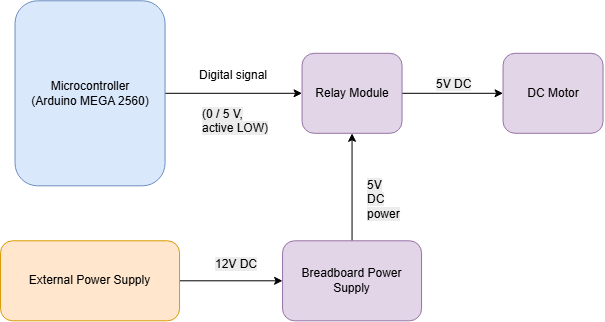
\includegraphics[width=1\linewidth]{img/diagrama_bloques-sistema7.drawio.png}
        \caption{Block Diagram of System 7.}\label{fig:15}
    \end{figure}

\end{enumerate}




\subsection{SYSTEM 8. Smart irrigation system}

\begin{enumerate}

    \item \textbf{Checkpoint 11: Carry out the physical implementation and record a demonstration video.}

    \begin{itemize}
        \item The physical implementation is demonstrated in the following video: 
        \href{https://drive.google.com/file/d/1GDMHu39VSYhLgZLV6vcsCYtYRBvduK-z/view?usp=drive_link}{view video demonstration}.
    \end{itemize}

    \item \textbf{Flowchart.}
    \par \vspace{0.15cm}
    Shown in Figure~\ref{fig:16}
    \begin{figure}[htbp]
        \centering
        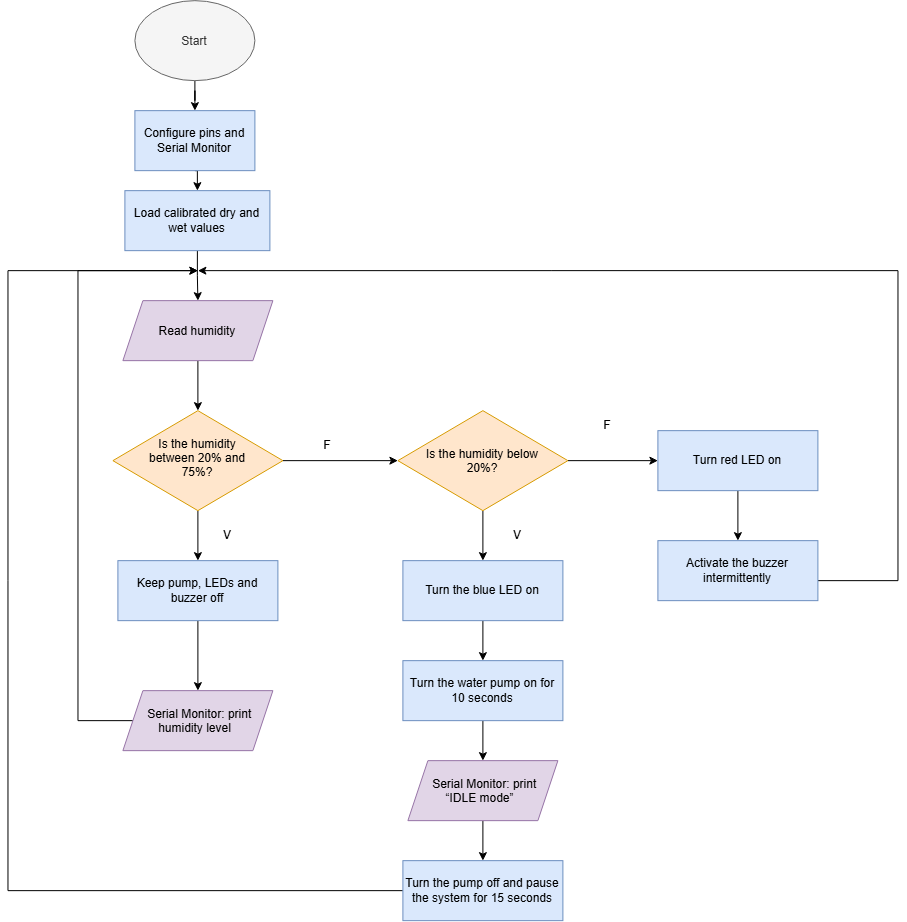
\includegraphics[width=1\linewidth]{img/diagrama_flujo-sistema8.drawio.png}
        \caption{Flowchart of System 8.}\label{fig:16}
    \end{figure}


    \item \textbf{Block Diagram.}
    \par \vspace{0.15cm}
    Shown in Figure~\ref{fig:17}
    \begin{figure}[htbp]
        \centering
        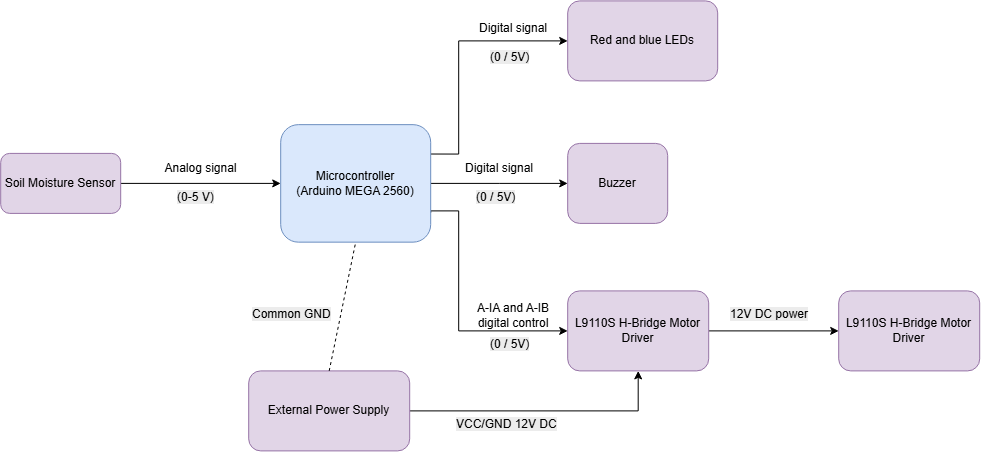
\includegraphics[width=1\linewidth]{img/diagrama_bloques-sistema8.drawio.png}
        \caption{Block Diagram of System 8.}\label{fig:17}
    \end{figure}

\end{enumerate}